\providecommand{\main}{../../..}
\providecommand{\Figures}{\main/Figures/Contraste}

\documentclass[\main/main.tex]{subfiles}

\begin{document}
            
\section{Méthodes d'amélioration de contraste au sein d'images 3D}

%
Comme vu précédemment, les images obtenues par un système d'imagerie peuvent présenter de fortes disparités de contraste, ayant différentes origines, et il n'est pas toujours possible de corriger tous les défauts lors de l'acquisition.
%
Il a donc été nécessaire de développer un certain nombre d'approches de corrections de contraste.
%
Je vais aborder trois sortes de méthodes permettant de compenser des défauts de contraste: des approches basées sur l'étude de l'histogramme des valeurs de gris, des approches basées sur la correction de la loi de Beer-Lambert et enfin des approches basées sur de multiplies acquisitions.

\subsection{Amélioration par égalisation d'histogrammes}

%%
%
Une des premières approches d'amélioration de contraste d'une image se basant sur l'analyse d'histogramme fut l'\he{}.
%
Cette méthode vise à "aplanir" l'histogramme des valeurs de gris de l'image.
%
En considérant la probabilité qu'un pixel ait une valeur inférieure ou égale à une certaine valeur de gris,
il est possible de calculer une fonction de répartition, qui attribuera à chaque valeur de gris une nouvelle valeur. De cette manière, le nouvelle histogramme aura une répartition plus homogène des valeurs de gris, ce qui permet en principe d'améliorer le contraste de l'image (voir Figure~\ref{fig:he}).

\begin{figure}[h]
    \centering
    \begin{subfigure}[b]{0.45\textwidth}
       \caption{
       Image d'origine
            }
       \centering 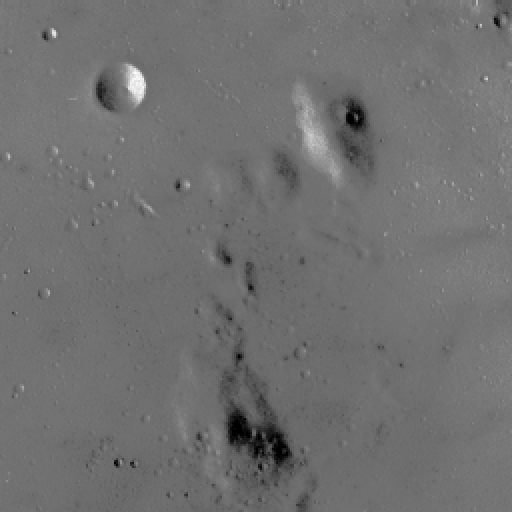
\includegraphics[width=\textwidth]{\Figures/moon.png}
    \end{subfigure}
    \begin{subfigure}[b]{0.45\textwidth}
       \caption{
       Après \he{}
            }
       \centering 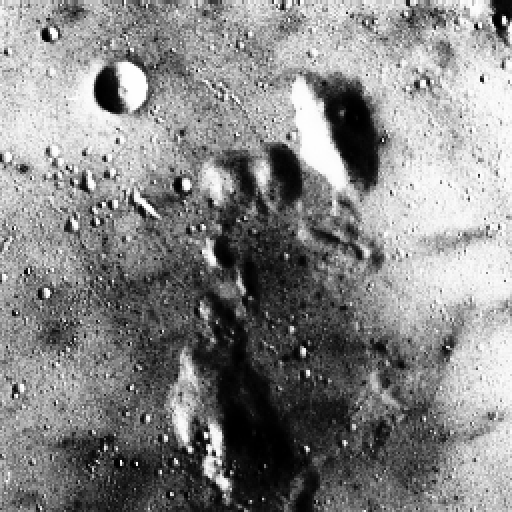
\includegraphics[width=\textwidth]{\Figures/moon_he.png}
    \end{subfigure}
    \caption{
        \label{fig:he}
        Exemple d'application d'une \he{}.
    }
\end{figure}


%%
%
Cependant, cette approche calculant les nouvelles valeurs de gris sur la base de l'histogramme des valeurs de gris de l'ensemble de l'image, cette approche ne tient pas compte du voisinage de chaque pixel. Cette approche ne sera par exemple pas en mesure de détecter un gradient de contraste au sein de l'image, ou une modification locale d'illumination.
%
Une correction de ce défaut a été apporté par le développement de l'\ahe{}\cite{hummel_1977}. Cette méthode consiste à calculer pour chaque pixel une fonction de répartition (voir Figure~\ref{fig:ahe}).
%
On choisit pour cela une forme représentant le voisinage de chaque pixel. L'\ahe{} calcule  la valeur de gris de chaque pixel en effectuant une \he{} au sein du voisinage. Cette approche locale permet ainsi de compenser des défauts liés à l'égalisation d'histogramme simple.
Cependant, cette approche est très sensible au bruit. En effet, le calcul de la fonction de répartition d'un pixel de bruit présent dans une région à intensité quasi-constante entraîne l'amplification du bruit.
%
La première solution proposé pour corriger ce défaut fut l'application d'un filtre Laplacien avant de calculer l'\ahe{}\cite{hummel_1977}. Malheureusement , cela peut altérer certaines structures de l'image d'origine, et ainsi faire perdre de l'information.

\begin{figure}[h]
    \centering
    \begin{subfigure}[b]{0.45\textwidth}
       \caption{
       Image d'origine
            }
       \centering 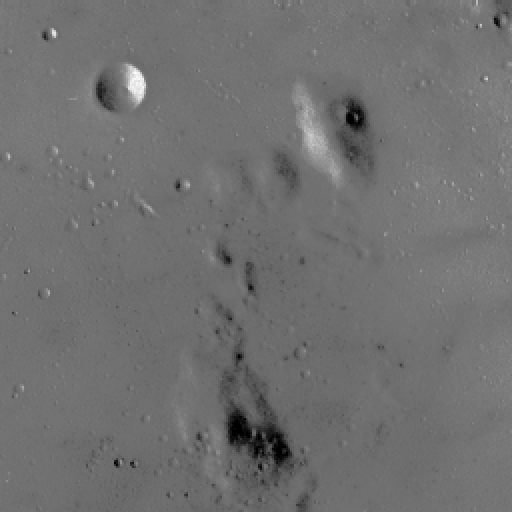
\includegraphics[width=\textwidth]{\Figures/moon.png}
    \end{subfigure}
    \begin{subfigure}[b]{0.45\textwidth}
       \caption{
       Après \ahe{}
            }
       \centering 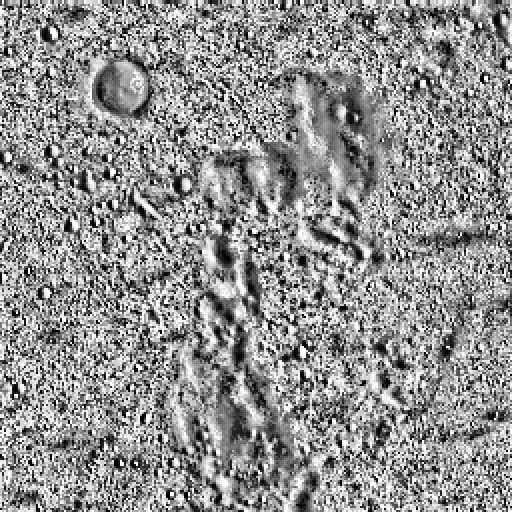
\includegraphics[width=\textwidth]{\Figures/moon_ahe.png}
    \end{subfigure}
    \caption{
        \label{fig:ahe}
        Exemple d'application d'une \ahe{}. Un noyau de 16 pixels a été choisi.
    }
\end{figure}
%%s
%
Une solution ultérieure fut le développement de l'\clahe{}\cite{pizer_1987}. Avant le calcul de l'\clahe{}, on définit une valeur seuil. L'histogramme des valeurs de gris pour chaque pixel est calculé et le nombre de pixels pour chaque valeur de gris est comparé à la valeur seuil choisie. Si une valeur de gris a un nombre de pixels supérieure à la valeur seuil, on redistribue cet excédant aux autres valeurs de gris. La fonction de répartition est alors calculée sur cet histogramme tronqué plutôt que sur l'histogramme d'origine (voir Figure~\ref{fig:clahe}).
%%
%
Pour une région quasi-constante, la redistribution des valeurs trop présentes transforme un histogramme présentant une région de pics en un histogramme plat. Ce changement de forme de l'histogramme permet de réduire l'amplification du bruit, car un pixel de bruit dans une zone constante ne sera plus détectable sur l'histogramme de répartition obtenue, et ne sera donc que peu modifié par l'application de la fonction de répartition.

\begin{figure}[h]
    \centering
    \begin{subfigure}[b]{0.45\textwidth}
       \caption{
       Image d'origine
            }
       \centering 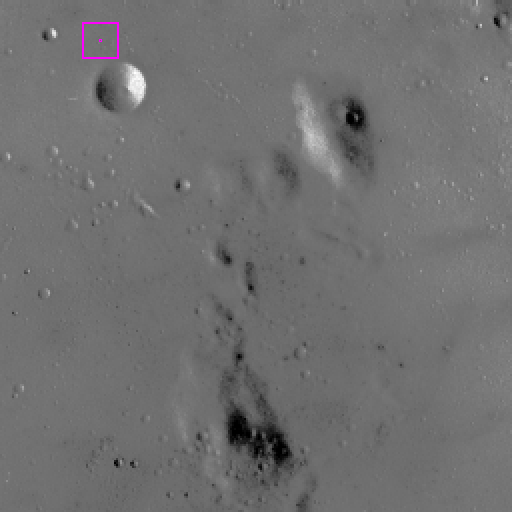
\includegraphics[width=\textwidth]{\Figures/moon_reveal.png}
    \end{subfigure}
    \begin{subfigure}[b]{0.45\textwidth}
       \caption{
       Après l'\clahe
            }
       \centering 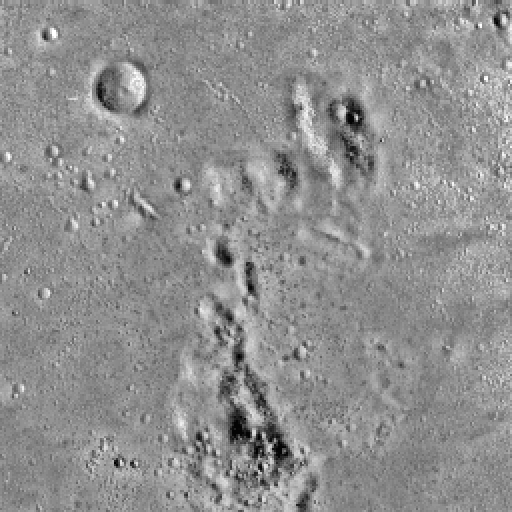
\includegraphics[width=\textwidth]{\Figures/moon_clahe.png}
    \end{subfigure}
    \begin{subfigure}[b]{0.45\textwidth}
       \caption{
       Histogramme local
            }
       \centering 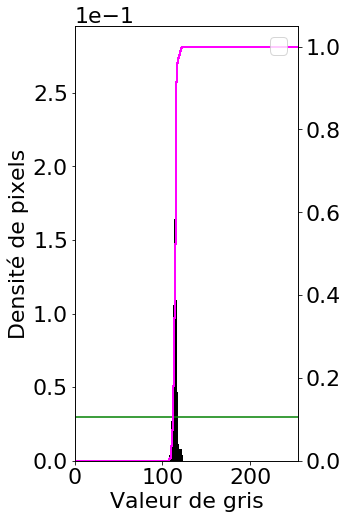
\includegraphics[width=\textwidth]{\Figures/hist_avant.png}
    \end{subfigure}
    \begin{subfigure}[b]{0.45\textwidth}
       \caption{
       \centering
       Histogramme local \\après limitation du contraste
            }
       \centering \includegraphics[width=\textwidth]{\Figures/hist_après.png}
    \end{subfigure}
    \caption{
        \label{fig:clahe}
        Exemple d'application de l'\clahe{}.
        Le cadre magenta représente la région utilisée pour calculer l'histogramme des valeurs de gris.
        Un noyau de 16 pixels et une valeur seuil de 0.03 ont été choisis.
        Pour les histogrammes, les ligne verte et  magenta représentent respectivement la valeur seuil et l'histogramme cumulé. 
    }
\end{figure}


\color{magenta}Ajouter figures explicative et d'illustration\color{black}

%%
%
Bien que publiée pour la première fois en 1987\cite{pizer_1987},
l'\clahe{} est encore largement utilisée\cite{dabass_2019,sonali_2018,lv_2019}.
%
En effet, il s'agit d'une méthode dont les principes sont simples à comprendre, ce qui la rend plus accessible et ce qui a mené à des développements supplémentaires très nombreux. Il est facile d'utiliser cet algorithme sans posséder de connaissances techniques pointues en analyse d'images.
%
Cette méthode a été largement implémentée dans différents logiciels de traitement d'images, comme \href{https://imagej.net/Enhance_Local_Contrast_(CLAHE)}{ImageJ},
\href{http://icy.bioimageanalysis.org/plugin/adaptive-histogram-equalization/}{icy} et \href{https://imagemagick.org/script/clahe.php}{imagemagik}.
%
Cependant, même si le grand nombre  de publications a rendu cette technique très populaire, elle possède néanmoins deux défauts majeurs.
%
Le premier est que l'\clahe{} demande un temps de calcul important.
%
En effet, le calcul de l'histogramme du voisinage de chaque pixel est une tâche lourde; et même si des algorithmes permettant de réduire les temps de calculs ont été proposés\cite{sund_2006}, l'utilisation de \clahe{} pour des images de grande taille n'a longtemps pas pu être réalisé dans un temps raisonnable sur des ordinateurs de bureau. De plus, la lourdeur des calculs ne permettait pas de traiter des imaes 3D jusqu'à récemment\cite{amorim_2018, stimper_2019}.
%%
%
Le second défaut est inhérent à la méthode employée.
%
En ne considérant que l'information fournie par l'image, ces algorithmes ne prennent pas en compte de potentiels défauts provenant de considérations physiques.
%
Cependant, d'autres méthodes ont été développés pour permettre de tenir compte de défauts provenant du système d'imagerie lui-même.

\subsection{Compensation de l'atténuation décrite par la loi de Beer-Lambert} % Il faut trouver une meilleur nom

%% Loi de Beer lambert
%
La loi de Beer-Lambert décrit l'absorption d'un faisceau lumineux en fonction de l'épaisseur de milieu traversé. Elle établit ainsi que l'absorption d'un rayon lumineux dans un milieu est proportionnelle à l'intensité lumineuse du rayon, la distance parcourue par ce rayon et la concentration de molécules responsables de l'atténuation.
%
Cette loi peut être décrite par la formule suivante:
\begin{equation}
    L(d) = L_{0}e^{-\kappa{}d}
\end{equation}
avec d la distance parcourue $L_{0}$ L'intensité lumineuse initiale, et $\kappa{}$ le coefficient d'absorption du milieu.

%
Cette loi est fréquemment utilisée en spectrophotomètrie. En fixant l'intensité lumineuse et la distance à parcourir, l'absorbance ne devient ainsi plus que fonction de la concentration.
%
Mais cette loi a aussi été utlisée des cadres très variées, comme l'évolution de l'état de santé des canopées\cite{demattos_2020, liu_2020a}, ou la mesure de la radiation stellaire.
% %
%
En traitement d'image, la compensation de la loi de Beer-Lambert permet d'améliorer le contraste d'une image en compensant la perte d'intensité lumineuse induite par le milieu. L'hypothèse de départ est alors que seul l'absorption est responsable de l'atténuation de la lumière dans le milieu,
négligeant ainsi l'importance de la diffusion ou de la diffraction.
%
Cependant, la loi de Beer-Lambert étant proportionnelle aux concentrations de molécules absorbantes, le coefficient d'atténuation est fonction de toutes les concentrations dans le milieu.
%
Utiliser la loi de Beer-Lambert est facile à réaliser dans un milieu contrôlé ne contenant qu'une molécule absorbante\cite{mikulewitsch_2018}. La modélisation de l'absorption devient cependant plus complexe dans des solutions contenant plus d'espèces de molécules, le coefficient d'absorption de la solution devenant la somme des coefficients d'absorption pour chaque espèce présente dans le milieu.
% %
%
Ansi, pour l'imagerie d'échantillons biologiques, tous les tissus ne vont pas contenir les mêmes concentrations d'espèces absorbantes. L'absorption ne peut donc pas être calculée pour une profondeur donnée, mais doit être calculée pour chaque colonne de voxels\cite{ohser_2020,nylk_2018,parker_2020}.
%
Ces approches demandent cependant une grande quantité de calcul,
car il est nécessaire d'effectuer une modélisation pour chaque colonne. Pour des images de grandes taille, le temps nécessaire à de tels calculs peut être trop long.
%%
%
Il est alors possible de compenser la loi de Beer-Lambert en multipliant les acquisitions.
%
Nous allons donc maintenant voir différentes solutions utilisant la multiplication des acquisitions.

\subsection{Approches par la multiplication d'acquisitions}

Plusieurs approches font appel à des acquisitions successives afin d'améliorer le contraste de l'image finale.
%

% %Vibe-Z
%
Vibe-Z\cite{ronneberger_2015} est un logiciel permettant d'étudier le cerveau de \pz{} à 72 hpf.
%
Pour ce faire, un modèle statistique de \pz{} a été créé en recalant les marquages au TOTO-3 de 85 échantillons.
%
Chaque échantillon présente en plus un contre marquage pouvant être une révélation par \fish{}, par \ihcie{} ou par l'emploi d'une lignée rapportrice. 
%
En appliquant à ce contre marquage la matrice de déformation employée pour recaler le marquage au TOTO-3 sur le modèle statistique, il est alors possible de connaître la position la plus statistiquement représentative de ce contre marquage.
%
Ceci permet ainsi de mettre en évidence de potentiels colocalisations sans effectuer de multiples marquages.

%
Vibe-Z comporte deux étapes d'améliorations de contraste basées sur l'utilisation de plusieurs acquisitions. La première étape consiste à comparer chaque acquisition avec une acquisition de la base de données du logiciel.
%
L'acquisition de référence est alors choisie pour être l'acquisition ayant le marquage le plus homogène au sein de la base de données.
%
Le coefficient d'atténuation de chaque voxel est alors calculé comme étant le quotient entre l'intensité de l'échantillon de référence et le coefficient de l'acquisition à améliorer.
%
Cette approche permet donc de corriger le contraste d'une image par l'emploi d'une image de référence.
%
Cependant, cette étape ne permet pas de compenser l'atténuation du signal en profondeur.
%
Cette correction est réalisé par la seconde étape, qui consiste à calculer le maximum par paire de voxel entre les deux acquisitions corrigées.
%
L'acquisition dorsale permet alors de compenser l'atténuation en profondeur de l'acquisition ventrale et inversement.
%
La fusion de deux acquisitions permet ainsi de corriger les défauts présents sur l'une d'entre elle.
%
En augmentant le  d'acquistions, il est alors possible d'améliorer le contraste de l'image finale.

%% Principe de la tomographie
%
La fusion de plusieurs acquisitions pour la formation d'une image finale est la base de la tomographie.
%
La tomographie consiste à calculer pour chaque voxel de l'image finale une valeur basée sur une série d'acquisitions 2D.
%
L'exemple le plus connu de tomographie est la tomodensitométrie\cite{hounsfield_1973}.
%
Au cours d'un examen tomodensitométrique, plusieurs acquisitions radiologiques sont effectués pour chaque plan de coupe de l'objet à analyser en effectuant une rotation autour de l'objet.
%
Chaque acquisition 2D pouvant être considérée comme une représentation de la somme des radiodensité pour un pixel,
il est possible de combiner ces acquisitions afin de créer une carte de radiodensité.
%
Une fois ces radiodensités calculées, on considère ces valeurs comme les valeurs de gris de l'image.
%
En reconstruisant l'image à partir d'une collection d'images 2D, il a ainsi été possible de reconstruire une image 3D dont le contraste ne varie que peu.
%
Cette méthode a ainsi été employée sur d'autres systèmes d'acquisitions.

%% rappel VAST
%
Comme présenté en section~\ref{sec:vast}, le VAST\cite{pardomartin_2010} est un système d'imagerie développé pour permettre l'\hti{} de \pz{}.
%
L'acquisition étant éffectuée par le biais de capillaire en verre, il n'est pas possible de réaliser d'imagerie 3D sans développer d'algorithme pour corriger les effets de lentilles induits par le capillaire.
%
Les seuls plans d'acquisition permettant d'éviter de phénomènes sont donc les plans se trouvant au centre du capillaire.
%
Cependant, ce système a été mis au point pour permettre d'effectuer des rotations du capillaire, et donc de l'échantillon à imager.

%% tomographie VAST
%
De cette manière, il est possible d'utiliser le VAST comme un système d'acquisition permettant de faire de la tomographie optique\cite{pardomartin_2013}, en effectuant plusieurs acquisition du même échantillon selon des angles différents.
%
En microscopie en champ clair,
cette approche a d'ailleurs été employée pour réaliser la volumétrie de la larve entière de \pz\cite{guo_2017}.
%
Mais son utilisation couplée à un système de microscopie confocale peut permettre une réalisation relativement simplem d'images 3D corriées par tomographie optique.

% % rappel SPIM
%
La microscope par nappe de lumière est une méthode de microscopie par fluorescence\cite{huisken_2004} (voir Section~\ref{sec:spim}).
%
L'illumination de la région à imager est effectuée par la création d'une nappe de lumière.
%
Il est ainsi possible d'illuminer toutes une région de l'échantillon, permettant ainsi d'accélerer l'acquisition tout en ayant une résolution axiale comparable à celle d'un microscope confocal.
%
Cependant, la feuille de lumière n'est générée que par une source unique.
%
Tout objet se trouvant ainsi sur le passage de la feuille de lumière peut induire une atténuation lumineuse.

%  % OPTISPIM
%
Une solution proposé est le développement d'un système permettant de réaliser une tomographie optique à partir de différentes acquisitions\cite{Mayer_2018}.
%
L'échantillon est alors placé sur une platine motorisée permettant de réaliser des rotations.
%
En permettant de réaliser l'acquisition 3D d'une même échantillon selon différents angles, il devient possible de réaliser une tomographie optique de l'échantillon.
%
Cette approche est intéressante car elle permet de faire une tomographie optique en se basant sur des données tridimensionnelles.

%% Critiques
%
Bien que ces approches permettent d'obtenir des images plus proches de la réalité biologique ou physique de l'échantillon étudié, les dispositifs nécessaires à ces acquisitions sont limitants.
%
Concernant de Vibe-Z, il est rare qu'un microscope dispose des deux objectifs permettant de réaliser l'imagerie d'une échantillon selon deux positions opposées.
%
Il est possible de réaliser l'imagerie des deux faces de l'échantillon séquentiellement en retournant l'échantillon, puis de recaler les deux acquisitions entre elle, mais la grande quantité de manipulations nécessaires rend cette solution incompatible avec le développement d'une plateforme d'\hti{}.
%
De la même manière, l'utilisation d'outils comme le VAST demande un système d'imagerie spécifique et peu versatile. Il est ainsi nécessaire de dédier un microscope uniquement à l'\hti{}, ce qui n'est pas forcément intéressant.
%
Enfin, OPTiSPIM étant basé sur la microscopie en nappe de lumière, il est difficilement possible de réaliser un montage permettant l'acquisition de plusieurs échantillons en une seule session d'imagerie.
%
Ces méthodes nécessitent pour la plupart de multiplier les acquisitions nécessaires à la réalisation d'une seule image, augmentant le temps dévolu à l'imagerie et au traitement de l'image.
% %
%
L'approche de l'amélioration de contraste par l'emploi de plusieurs acquisitions semble en résumé peu compatible avec le développement d'une plateforme de \hcs{}.


\end{document}
